% chktex-file 1
% chktex-file 8
% chktex-file 24
% chktex-file 36
% chktex-file 44

\chapter{Umstrukturierung und Innovation}

Als erstes gilt es herauszufinden welcher Teil des Code, der zuständig für das Prompting ist, 
wie verbessert werden kann.
Das Projekt von Weidl\cite{weidl2024bpmngen} und Shi\cite{shi2025bpmngen} benutzt zur Erstellung 
von BPMN Diagrammen die OpenAI API und verwendet hier die Technologie der Assistants\@.
\footnote{\url{https://platform.openai.com/docs/assistants/overview}}

\section{Generelle Umstrukturierungen}

Während der Code gut für seinen (bisherigen) speziellen Anwendungsfall ist, können hier einige 
Verbesserungen gemacht werden.

\subsection{Objektorientierter Ansatz}

Das Zeil ist es, den Code einfach erweiterbar und wartbar zu machen.
Hierfür ist es wichtig, den code möglichst schnell an Änderungen der OpenAI Api anpassen zu können.
Um das zu erreichen wird ein Objektorientierter Ansatz gewählt.
Die objektorientierte Programmierung bietet für den Aufbau des Prompting-Codes viele Vorteile und macht die Entwicklung 
langfristig übersichtlicher und wartbarer. 
Wir erstellen eine abstrakte Klasse \texttt{Ai} welche die gesamte Logik des Prompting beinhält und eine Klasse \texttt{ChatGPT} 
welche von der AI Klasse erbt.
Die ChatGPT Klasse muss nun nur noch Methoden implementieren, welche konkret auf die aktuelle version der API angepasst sind.
Durch die Verwendung von abstrakten Methoden wie \mintinline{typescript}{generateContent()}, 
\mintinline{typescript}{createTitle()} oder processResponse() wird sichergestellt, 
dass jede konkrete Implementierung dieselbe Schnittstelle einhält, 
aber ihre eigenen internen Abläufe definieren kann. 
Dies erleichtert den Austausch und die Erweiterung von Modellen, ohne den restlichen Code verändern zu müssen. 
Darüber hinaus werden wiederkehrende Prozesse, etwa das Speichern von Verläufen, das Verarbeiten von Antworten 
oder die Konvertierung zwischen Formaten, zentral in der Basisklasse gekapselt. 
Falls sich die API ändert, kann dies nun einfach in der Erbenden Klasse angepasst werden, ohne die dahinterliegenden Logik verändern zu müssen.

So sieht nun in abgespeckter Variante die Klasse für die OpenAI API aus.
Es gibt eine Methode \mintinline{typescript}{mapPromptInput();} um den Prompt in das richtige Format der API zu bringen,
\mintinline{typescript}{generateContent();} um den eigentlichen API aufruf durchzuführen und \mintinline{typescript}{preocessResponse();}
um die Antwort der API auszulesen.

\begin{code}
\begin{minted}[frame=single, framesep=2pt, linenos, fontsize=\small, style=vs]{typescript}
export class ChatGPT extends Ai {
  openai = new OpenAI({
    apiKey: OPENAI_API_KEY,
  });
  assist = await openai.beta.assistants.retrieve("asst_...");

  protected mapPromptInput(input) {
    return {
      input: input.prompt,
      model: this.model,
    };
  }

  protected async generateContent(input) {
    return await openai.beta.threads.runs.createAndPoll(
      thread_id, 
      { assistant_id: assist.id },
      { role: "user", content: input }
    );
  }

  protected processResponse(response) {
    return response.output_text.toString();
  }
}
\end{minted}
\caption{ChatGPT Klasse}\label{code:chatgpt-class}
\end{code}

\subsection{Von Assistants zu Responses}

Die Änderungen welche im vorherigen Kapitel beschrieben wurden, zeigen gleich ihren Effekt, 
da OpenAI ankündigt ihre Assistants API einzustellen.
Sie emfehlen einen Umzug zu einer ihrer neueren APIs\@.
Für dieses Projekt wird die Responses API gewählt
\footnote{\url{https://platform.openai.com/docs/api-reference/responses}}
\footnote{\url{https://platform.openai.com/docs/assistants/migration}}.
Dies ist nun recht einfach umzusetzten, da wir nur die elementaren Methoden der API ändern müssen. 
Wie nun zum Beispiel die neue Methode \mintinline{typescript}{generateContent();} für die
Responses API aussieht, kann man in Abbildung~\ref{code:generate-content} sehen.

\begin{code}
\begin{minted}[frame=single, framesep=2pt, linenos, fontsize=\small, style=vs]{typescript}
protected async generateContent(input) {
  return this.openai.responses.create(input);
}
\end{minted}
\caption{generateContent()}
\label{code:generate-content}
\end{code}

Einer der zentralen Unterschiede zwischen der Assistants- und der Responses-API besteht darin, 
dass die System-Instructions bei der Verwendung der Responses-API manuell übergeben werden müssen. 
Dadurch ist es notwendig, die entsprechenden Anweisungen bei jeder Anfrage erneut mitzusenden. 
Dies bringt jedoch nicht nur zusätzlichen Aufwand mit sich, sondern eröffnet auch neue Möglichkeiten: 
Die Instructions können flexibel und situationsabhängig angepasst werden, wodurch sich das Verhalten des Modells 
dynamisch steuern lässt.
Im folgenden Abschnitt wird gezeigt, wie dieser Ansatz weiter verbessert und effizienter gestaltet werden kann.

\subsection{Verbesserung der instructions}

Da die Instructions nun manuell mit jeder Anfrage übergeben werden, bietet sich die Möglichkeit, deren Aufbau 
gezielt zu optimieren. 
Ziel dieser Optimierung ist es, die Anzahl der benötigten Input-Tokens zu reduzieren, ohne dabei Qualität einzubüßen. 
Im besten Fall wird die Ausgabequalität sogar verbessert.
Der Assistant erhält als Grundlage zwei PDF-Dateien, die BPMN-Diagramme und den BPMN 2.0 
Standard im Detail beschreiben, sowie zwei Textdateien: 
Eine mit der Definition des verwendeten JSON-Formats und eine mit allgemeinen Regeln zum Aufbau der Diagramme. 
Die beiden PDF-Dokumente umfassen zusammen mehr als 10 MB und über 100 Seiten Text. 
Da ChatGPT bereits ein solides Grundverständnis von BPMN-Diagrammen besitzt, werden diese umfangreichen Dateien aus 
den Instructions entfernt. 
Mehrere Tests zeigen, dass sich diese Reduktion nicht negativ auf die Ergebnisqualität auswirkt. TODO
Dadurch lassen sich eine große Zahl an Tokens sowie Rechenzeit und Kosten einsparen.

Die beiden verbliebenen Textdokumente werden anschließend zusammengeführt und in ein einheitliches, 
strukturiertes Format gebracht. 
Alle Regeln sind in einer geordneten Liste zusammengefasst und durch \texttt{Structured-Prompting} klar und 
maschinenlesbar gestaltet. 
Ergänzend werden den Instructions zwei illustrative Beispiele hinzugefügt:
Zum einen ein minimales Beispiel, das den grundsätzlichen Aufbau des JSON-Formats verdeutlicht und die 
obligatorischen Elemente zeigt. 
Zum anderen ein umfangreicheres, praxisnahes Beispiel, das ein vollständiges BPMN-Diagramm mit allen relevanten und 
unterstützten Komponenten abbildet. 
Dieses \texttt{Few-Shot-Prompting}, oder in diesem Fall \texttt{Two-Shot-Prompting}, sorgt dafür, dass der Assistant sowohl 
einfache als auch komplexe Diagramme interpretieren und reproduzieren kann.
Diese Technik ist auch bereits bei anderen BPMN Chatbots getestet worden und hat sich als sinnvoll erwiesen.
~\cite{koeppke2025BPMNChatbotPP,kourani2024promoai,ziche2024llm4pm}

\section{Formatauswahl}

Bisher wird die KI angewiesen, das Diagramm in einem eigens definierten JSON-Format zu erzeugen. 
Dieses Format wurde jedoch speziell für diesen Anwendungsfall entworfen und existiert in dieser Form nicht offiziell.
Entsprechend konnte das Modell während des Trainings kein Vorwissen darüber erwerben, sondern muss das Format 
ausschließlich auf Grundlage der bereitgestellten Instructions erlernen. 
Dadurch besteht die Möglichkeit, dass Fehler auftreten, etwa dann, wenn die Anweisungen unvollständig sind oder dem Modell 
bestimmte Kontextinformationen fehlen.

Um dieses Problem zu vermeiden, wird künftig die Option ergänzt, dass die KI ihre Ausgabe auch direkt im offiziellen 
Standardformat erzeugen kann. 
Das Standardisierte Format für BPMN 2.0 Diagramme ist XML, 
zu dem umfangreiche Dokumentationen und etablierte Werkzeuge existieren.\cite{omg2014bpmn2}
Dennoch bietet das eigens entwickelte JSON-Format einen entscheidenden Vorteil: 
Es besitzt eine deutlich höhere Informationsdichte und lässt sich dadurch schneller und effizienter verarbeiten.
Aus diesem Grund haben sich einige anderen Implementierungen eines Text zu BPMN durch LLM dafür entschieden ein Zwischenformat
wie das hier genannte JSON zu verwenden.
Dazu gehört AutoBPMN.AI~\cite{klievtsova2015autobpmnai} welche auf das Format Mermaid gesetzt haben oder
NaLa2BPMN~\cite{noureldin2024nala2bpmn} welche auch ein JSON implementieren.
Beide Varianten, sowohl das direkte vollständige generiren als auch die Generierung mit Zwischenmodell, 
haben ihre jeweiligen Stärken und Schwächen.
Diese sind in Tabelle~\ref{tab:vor-nachteile-json-xml} zu sehen.

\begin{table}[H]
  \centering
  \renewcommand{\arraystretch}{1.2}
  \begin{tabular}{|p{2cm}|p{5.5cm}|p{5.5cm}|}
    \hline
    \textbf{} & \textbf{JSON-Format} & \textbf{XML-Format} \\ \hline
    \textbf{Vorteile} &
    hohe Informationsdichte,\newline geringer Tokenverbrauch,\newline schnelle Generierung. &
    Standardisiert,\newline gut dokumentiert,\newline weit verbreitet,\newline einfachere Instructions \\ \hline
    \textbf{Nachteile} &
    Kein Standard,\newline Lernaufwand,\newline komplizierter Konvertierungsalgorythmus. &
    hoher Tokenverbrauch,\newline umfangreiche Syntax,\newline unübersichtlicher,\newline mehr Kosten,\newline längere Generierung.\\\hline
  \end{tabular}
  \caption{Vergleich der Vor- und Nachteile der unterstützten Ausgabeformate}
\label{tab:vor-nachteile-json-xml}
\end{table}

Für die Weiterentwicklung ist ein flexibles System das Ziel, das eine dynamische Auswahl des Ausgabeformats besitzt. 
Dadurch kann der Nutzer selbst entscheiden, welches Format im jeweiligen Anwendungsfall die besseren Ergebnisse liefert. 
Da sich die Formatwahl ähnlich wie die Wahl des verwendeten Modells direkt auf die Qualität der Ergebnisse auswirkt, 
wird die Auswahlmöglichkeit direkt in die Modellkonfiguration integriert. 
So kann beispielsweise zwischen Varianten wie `gpt-4.1-mini (xml)' und `gpt-4.1-mini (json)' gewählt werden. 
Alternativ kann das Format such im separaten \texttt{format} Parameter angegeben werden.
Wird kein Format angegeben, erfolgt die Ausgabe standardmäßig im XML-Format.

Eine Anfrage sieht damit z.B. aus wie in Codeausschnitt~\ref{code:post-model-format}.

\begin{code}
\begin{minted}[frame=single, framesep=2pt, linenos, fontsize=\small, style=vs]{json}
// POST /threads
{ 
  "inputString": "Bitte generiere mir ein BPMN Diagram, 
      welches den Ablauf in einem Restaurant zeigt", 
  "model": "gpt-5 (xml)",
  "format": "xml"
}
\end{minted}
\caption{Post Request an /threads mit Format}
\label{code:post-model-format}
\end{code}

Bei einer Anfrage kann dann die jeweilige AI über eine Map 

\mintinline{typescript}{const availableGPTs: Map<string, Ai>} 

zugeordnet werden, welche die Anfrage bearbeitet.

\paragraph{Diagrammupdates}

Die erstellten Diagramme bearbeiten zu lassen, ist ein wesentlicher Bestandteil der Software.
Weidel~\cite{weidl2024bpmngen} hat das Update des Diagramms so implementiert, dass ein JSON Block
an das generierte Diagramm anghängt wird.
In diesem Block sind die Änderungen definiert, während der Text der eigentlichen Diagrammgenerierung nicht verändert wird.
Obwohl Veränderungen so sehr schnell generierbar sind, hat es leider auch manche Nachteile.
Zum einen wird somit die Datei, welche auch immer an die KI mitgesendet werden muss, immer länger,
wodurch auch die Anzahl an Input Tokens immer weiter steigt.
Zum anderen ist es nicht möglich, dass der Nutzer manuell Änderungen an dem Diagramm vornehmen kann
und die KI dann mit diesen Änderungen fortfährt.

Ausserdem ist ein solcher Update Block nicht im offiziellen XML Standard definiert. 
Daher kann diese Technik nicht angewendet werden auf direkte XML-Diagramm Erstellungen.
Für den weiteren Verlauf wird daher das Verfahren der Update Blöcke entfernt und stattdessen wird bei
einer Diagrammänderung das gesamte Diagramm neu generiert.
\footnote{Mehr dazu im Abschnitt~\ref{sec:konversationskontext}}
Einer KI die Möglichkeit zu geben, ihre vorherigen Fehler zu aus dem Diagramm vollstänig zu beheben,
kann sinnvoll sein, da dadurch jeglicher Fehler korrigiert werden kann und die KI zum Beispiel auch wieder Teile 
entfernen kann, ohne dass die Diagrammdefinition länger wird.
Dies haben auch andere ähnliche Projekte so entscheiden.~\cite{klievtsova2015autobpmnai,koeppke2025BPMNChatbotPP}

Im Folgenden soll gezeigt werden, dass die Qualität durch die gemachten veränderungen nicht nachgelassen hat.
Dafür wird ein Diagramm sowohl für den alten Assistant als auch für die gemachten Änderungen erstellt.
Für beide wird der einheitliche Prompt 1.3 aus dem PET Dataset~\cite{bellan2022pet}, sowie GPT-4.1 verwendet.

\noindent\fbox{
  \parbox{.96\textwidth}{
    The Evanstonian is an upscale independent hotel. When a guest calls room service at The Evanstonian, 
    the room-service manager takes down the order. She then submits an order ticket to the kitchen to 
    begin preparing the food. She also gives an order to the sommelier (i.e., the wine waiter) to fetch 
    wine from the cellar and to prepare any other alcoholic beverages. Eighty percent of room-service 
    orders include wine or some other alcoholic beverage. Finally, she assigns the order to the waiter. 
    While the kitchen and the sommelier are doing their tasks, the waiter readies a cart (i.e., puts a 
    tablecloth on the cart and gathers silverware). The waiter is also responsible for nonalcoholic 
    drinks. Once the food, wine, and cart are ready, the waiter delivers it to the guest`s room. After 
    returning to the room-service station, the waiter debits the guest`s account. The waiter may wait 
    to do the billing if he has another order to prepare or deliver.
  }
}

Die generierten Diagramme sind in den Abbildungen~\ref{fig:dia-assistant},~\ref{fig:dia-responses-json} und
~\ref{fig:dia-responses-xml} zu sehen.
Wie man erkennen kann, wurde die Qualität durch die Änderungen sogar verbessert.

\section{Dateien}

Um die Qualität des Promptings weiter zu verbessern, soll eine Funktionalität implementiert werden, 
die es ermöglicht, auch Dateien direkt an die KI zu übermitteln. 
Dabei steht im Vordergrund, dass das Verfahren sowohl im Frontend als auch im Backend möglichst 
unkompliziert umgesetzt werden kann. 
Es soll keine aufwendigen oder zeitraubenden Konvertierungen erfordern und eine breite Auswahl an 
Dateitypen unterstützen, um die Nutzung so flexibel wie möglich zu gestalten.
Nach einer Analyse der OpenAI-Dokumentation
\footnote{\url{https://platform.openai.com/docs/guides/images-vision?api-mode=responses&format=base64-encoded}}
zeigt sich, dass die einfachste und zugleich effizienteste Methode zur Dateiübertragung die 
Verwendung einer Base64 Data URL ist. 
Diese Variante bietet eine einfache Möglichkeit, Binärdaten wie Bilder oder Dokumente direkt 
in Textform zu kodieren und zu übermitteln, ohne zusätzliche Infrastruktur oder spezielle 
Upload-Mechanismen zu benötigen.

Eine Base64 Data URL ist eine Textdarstellung einer Datei, die direkt in eine URL eingebettet wird. 
~\cite{rfc2397,rfc4648}
Dabei werden die ursprünglichen Binärdaten in ein spezielles Textformat namens Base64 umgewandelt. 
Diese kodierten Daten beginnen typischerweise mit einer Kennzeichnung wie data:image/png;base64,\dots 
und enthalten danach die eigentlichen kodierten Inhalte. 
Der große Vorteil liegt darin, dass der Browser oder die API diesen Text einfach wieder in die 
ursprüngliche Datei zurückwandeln kann. 
Auf diese Weise lassen sich Dateien direkt in 
JSON API-Anfragen integrieren, ohne dass zusätzliche Anfragen oder externe Speicherorte 
erforderlich sind. 
Dieses Verfahren ist daher besonders gut geeignet, um eine einfache, schnelle und universell 
kompatible Dateiübertragung zu ermöglichen.
AUsserdem wird diese Formatierung von allen relevanten LLM Anbietern unterstützt.
Dadurch, dass die Datei nun einfach als String übergeben werden kann, können wir die Datei dem Body 
der Anfrage hinzufügen.

Eine Anfrage sieht damit z.B. wie in Codeausschnitt~\ref{code:post-file} aus.
Der string wird dann in Codeausschnitt~\ref{code:check-base64} auf Validität geprüft
und dann wie in Codeausschnitt~\ref{code:chatgpt-file-format} im richtigen Format an 
die OpenAI API gesendet:

\begin{code}
\begin{minted}[frame=single, framesep=2pt, linenos, fontsize=\small, style=vs]{json}
// POST /threads
{ 
  "inputString": "Bitte generiere mir ein BPMN Diagram, 
      welches den Ablauf in einem Restaurant zeigt", 
  "model": "gpt-5 (xml)",
  "file": "data:image/png;base64,A35ekZ...",
}
\end{minted}
\caption{Post Request an /threads mit Datei}
\label{code:post-file}
\end{code}

\begin{code}
\begin{minted}[frame=single, framesep=2pt, linenos, fontsize=\small, style=vs]{typescript}
private checkBase64DataUrl(dataUrl: string): boolean {
  regex = /^data:([\w.+-]+\/[\w.+-]+)?;base64,[\w+\/]+=*$/;
  return regex.test(dataUrl);
}
\end{minted}
\caption{checkBase64DataUrl()}
\label{code:check-base64}
\end{code}

\begin{code}
\begin{minted}[frame=single, framesep=2pt, linenos, fontsize=\small, style=vs]{typescript}
const imageInstructions = {
  role: "user",
  content: [
    {
        type: "input_file",
        file_url: input.getFileDataUrl() as string,
    } as ResponseInputFile,
  ],
} as ResponseInputItem
\end{minted}
\caption{Darstellung des Formats für die ChatGPT API}
\label{code:chatgpt-file-format}
\end{code}

\section{Chain of Thought}

Um die Erzeugung und Interaktion rund um BPMN-Diagramme weiter zu verbessern, wird eine 
Technik implementiert, die als \texttt{Chain of Thought}\cite{wei2023chainofthought} bekannt ist. 
Dieses Verfahren ermöglicht es dem Modell, komplexere Denkprozesse intern nachzuvollziehen und 
schrittweise zu argumentieren, bevor eine Antwort erzeugt wird. 
Dadurch kann der Dialog natürlich und strukturiert verlaufen, da der Chatbot in der Lage ist, 
Zusammenhänge besser zu verstehen und über mehrere Gesprächsschritte hinweg Ergebnisse 
zu liefern.

Diese Erweiterung erlaubt es dem Nutzer, auf vielfältige Weise mit dem Chatbot zu interagieren: 
Es können Fragen gestellt werden, Ideen vorgeschlagen, bestehende Diagramme erläutert oder 
Verbesserungsvorschläge erfragt werden. 
Der BPMN-Bot soll damit nicht nur ein Werkzeug für Diagrammerstellung bleiben, sondern sich zu einem 
vollwertigen Assistenten weiterentwickeln, der beim gesamten Modellierungsprozess 
unterstützt.

Darüber hinaus ist vorgesehen, dass der Chatbot selbstständig Rückfragen stellt, wenn bestimmte 
Angaben unvollständig, mehrdeutig oder widersprüchlich sind. 
So kann ein interaktiver Dialog entstehen, in dem beide Seiten zum Verständnis und zur Qualität 
des Diagrammes beitragen. 
Um dies zu ermöglichen, benötigt der Chatbot Zugriff auf den bisherigen Gesprächsverlauf sowie auf 
den aktuellen Zustand des jeweiligen Diagrammes. 
Nur durch diese Kontextkenntnis kann die KI sinnvolle 
Antworten generieren.

\subsection{Implementierung eines neuen Modus}

Um die Erstellung von Diagrammen für den Nutzer nicht unnötig zu verkomplizieren,
bleibt die direkte Generierung eines BPMN-Diagramms weiterhin bestehen. 
Gleichzeitig soll jedoch mehr Flexibilität bei der Art der Interaktion geboten werden. 
Zu diesem Zweck wird der Anfrage ein zusätzlicher Parameter hinzugefügt, 
der das Antwortverhalten der KI steuert.

Über den Parameter \texttt{mode} kann festgelegt werden, in welchem Modus die
KI reagieren soll. 
Der bisherige Modus, bei dem ausschließlich das Diagramm
erzeugt wird, trägt nun die Bezeichnung \texttt{quick}. 
In diesem Modus erfolgt die Ausgabe direkt und ohne weiteren Dialog.

Der neu eingeführte Modus \texttt{detail} aktiviert den Chain of Thought-Ansatz. 
In diesem Modus verhält sich die KI dialogorientiert.
Sie kann Rückfragen stellen, Überlegungen anstellen oder alternative Vorschläge
anbieten, bevor das endgültige Diagramm erstellt wird. 
Dadurch entsteht eine interaktive Konversation, die vor allem bei komplexeren Prozessen oder
unvollständigen Eingaben von Vorteil ist.

Eine Anfrage, die eine solche erweiterte Unterhaltung ermöglicht, könnte
beispielsweise wie in Codeausschnitt~\ref{code:post-mode} aussehen:

\begin{code}
\begin{minted}[frame=single, framesep=2pt, linenos, fontsize=\small, style=vs]{json}
// POST /threads
{ 
  "inputString": "Bitte schlag drei Prozessbeschreibungen 
    vor, aus denen dann eine ausgewählt wird um ein Diagramm
    zu erstellen.", 
  "model": "gpt-5 (xml)",
  "mode": "detail",
}
\end{minted}
\caption{Post Request an /threads mit mode}
\label{code:post-mode}
\end{code}

\subsection{Konversationskontext} \label{sec:konversationskontext}

Da es nun darum geht einen Chat zu implementieren, bei dem die KI möglichst gut auf Nachrichten reagieren
kann, ist es wichtig, dass die KI Zugriff auf vorherige Nachrichten sowie auf das aktuellste Diagramm hat.
Wäre das nicht der Fall, könnte die KI keine Fragen über das Diagramm beantworten und auch keine 
richtige Unterhaltung führen, da immer nur die aktuellste Nachricht vorhanden ist.
Bei LLM Anbietern wie OpenAI ist es notwendig, dass die Nachrichtenhistorie in der Anfrage 
mitgeschickt wird.

Hierfür müssen alle Nachrichten eines Threads aus der Datenbank geladen werden.
Die Nachrichten werden dann auf das Wesentliche gefiltert und auf ein kompaktes Format gebracht.
Die OpenAI Klasse muss dann nur noch die Nachrichten auf das von der API geforderte Format bringen und in der
Anfrage mitschicken.

Da die Anfagen an die KI immer komplexer werden, wird nun eine Klasse \texttt{PromptInput} angelegt.
Diese Klasse beinhaltet alle Informationen welche der KI mitgesendet werden sollen.
Bei einer Erstellung dieses Objekts können alle Rohdaten wie Instructions, Dateien oder der Chatverlauf
übergebe werden, welche die Klasse dann automatisch formatiert.
Ein entscheidender Schritt hierbei ist es die Teile der Nachrichten zu entfernen, in denen die KI mit einem
Diagramm geantwortet hat.
Das ist wichtig, da die Diagramme viele Tokens beinhalten und eigentlich nur das aktuellste Diagram 
wichtig ist. Hier bei kann es aber auch sein, dass das Diagramm noch vom Nutzer bearbeitet wurde.
Um dies zu berücksichtigen sind die Diagramme nicht Teil der Nachrichten, welche mitgesendet werden.
Die Implementierung der KI-Schnittstelle kann anschließend ein Objekt der Klasse \texttt{PromptInput} 
entgegennehmen. 
Dieses Objekt dient als zentrale Datenstruktur, über die alle für die Anfrage relevanten Informationen 
an das Modell übergeben werden. 
Mithilfe vordefinierter Hilfsmethoden lässt sich der Inhalt komfortabel in das gewünschte 
Eingabeformat konvertieren, sodass keine manuelle Aufbereitung mehr erforderlich ist.

Die Klasse \texttt{PromptInput} verfügt über die in Abbildung~\ref{code:promptinput-class} zu sehenden 
Attribute.

\begin{code}
\begin{minted}[frame=single, framesep=2pt, linenos, fontsize=\small, style=vs]{typescript}
export class PromptInput {
  instructions: string[];
  history: {role: "user" | "assistant", content: string}[];
  prompt: string;
  file?: string;
}
\end{minted}
\caption{PromptInput Klasse}
\label{code:promptinput-class}
\end{code}

Damit ist es möglich, bestehende Nachrichtenverläufe aus der Datenbank abzurufen und automatisch in 
das benötigte Format zu überführen. 
Die Klasse übernimmt hierbei die vollständige Strukturierung der Daten, sodass diese
für die Kommunikation mit der KI genutzt werden können:

\begin{code}
\begin{minted}[frame=single, framesep=2pt, linenos, fontsize=\small, style=vs]{typescript}
const instructions = [formatInstructions, modeInstructions];
const chatsFromDB = getAllChatsFromDB(threadID);
new PromptInput(instructions, prompt, chatsFromDB, file);
\end{minted}
\caption{PromptInput Erstellung}
\label{code:prompt-input-creation}
\end{code}

Das so erzeugte \texttt{PromptInput}-Objekt kann anschließend durch interne Methoden in das finale 
Format umgewandelt werden, das von der KI-Schnittstelle erwartet wird. 
Dadurch entsteht ein einheitlicher, wiederverwendbarer Datenfluss zwischen Anwendung, Datenbank und 
Modell, der die Wartung sowie zukünftige Erweiterungen vereinfacht.

\begin{code}
\begin{minted}[frame=single, framesep=2pt, linenos, fontsize=\small, style=vs]{typescript}
protected mapPromptInput(input: PromptInput) {   
  [...]
  const historyInstructions = input.history.map((item) => {
    return {role: item.role, content: item.content};
  });
  return {
    input: [systemInstructions, historyInstructions, 
            userInstructions, fileInstructions],
    model: this.model,
  };
}
\end{minted}
\caption{mapPromptInput()}
\label{code:map-promptinput}
\end{code}

Darüber hinaus soll künftig auch die jeweils aktuellste Version des Diagramms an die Anfrage angehängt 
werden. 
Auf diese Weise erhält die KI den vollständigen Kontext und kann das bestehende Diagramm nicht nur 
bearbeiten, sondern auch inhaltliche Fragen dazu beantworten.

Da das aktuelle Diagramm nicht Bestandteil des eigentlichen Nachrichtenverlaufs ist, wird es in den 
System Instructions hinterlegt. 
Dieser Block wird nun als `Update Instruction' bezeichnet und enthält stets die zuletzt 
gespeicherte Version des Diagramms. 
Die entsprechenden Daten werden automatisch aus der Datenbank geladen und vor dem Absenden der Anfrage 
in die System Instructions eingefügt.
Dies ist in Codeausschnitt~\ref{code:update-instructions} zu sehen.

Durch dieses Verfahren ist sichergestellt, dass die KI bei jeder Interaktion auf dem neuesten Stand 
bleibt und Änderungen im Diagramm jederzeit konsistent nachvollziehen kann.

\begin{code}
\begin{minted}[frame=single, framesep=2pt, linenos, fontsize=\small, style=vs]{typescript}
protected updateInstructions(threadID: string, format: format){
  const diagram = getLatestDiagramFromDB(threadID);
  return [`The The following diagram has already been created:
    ${format == "xml" ? diagram?.xml : diagram?.json}`]
}
\end{minted}
\caption{updateInstructions()}
\label{code:update-instructions}
\end{code}

Damit hat die KI nun alle Informationen die sie benötigt um eine Konversation führen zu können.

\subsection{Konversationen} \label{sec:konversationen}

Für eine vollständige Konversation benötigt die KI nun aber noch Anweisungen.
Dafür werden der KI noch ein weiterer Block Instructions hinzugefügt.
Diese werden als `Update Instructions' bezeichnet.
Diese sehen zunächst so aus:

\begin{minted}[frame=single, framesep=2pt, linenos, fontsize=\small, style=vs]{text}
[Output Language depends on prompt language]

Instead of creating a bpmn diagram, you can also chat with the 
user.
Any descriptions, questions, summaries or any other type of 
text the user may want, you must answer.
You may ask any questions you feel like you need to 
answer to create the best bpmn diagram.
If you do not have any questions anymore, you may write a 
quick summary of the agreed diagram before creating the 
bpmn.
If the initial prompt is really basic, provide the user with a 
creative scenario summary.

If you want to provide questions, summary or any other type of 
text, that is not a diagram. Do not use JSON or XML. 
Only plain Text!
You may answer with both a plaintext section and a diagram. 
Do not put plain text in a JSON or XML section. 
If you want to provide a description, summary or any other type 
of text, that is not a diagram, send it outside the diagram.
\end{minted}

Diese Instructions werden nur mitgesendet, falls der \texttt{detail} modus genutzt wird.

Wenn man den Bot nun fragt: ``Bitte schlag mir ein Diagramm vor'', hat dieser geantwortet mit:

\setlist{nolistsep}
\noindent\fbox{
  \parbox{.96\textwidth}{
    Gerne, ich schlage Ihnen ein klassisches und leicht verständliches Szenario vor: 
    einen \textbf{Online-Bestellprozess}. 
    Dieses Diagramm würde die Interaktion zwischen einem Kunden und einem Online-Shop 
    darstellen und eignet sich gut, um grundlegende BPMN-Konzepte zu zeigen. 
    \textbf{Zusammenfassung des vorgeschlagenen Diagramms:} 
    \begin{itemize}[noitemsep]
      \item \textbf{Beteiligte (Pools):}
        \begin{enumerate}[noitemsep]
          \item Kunde
          \item Online-Shop
        \end{enumerate}
      \item \textbf{Ablauf beim Kunden:}
        \begin{enumerate}[noitemsep]
          \item Der Prozess beginnt damit, dass der Kunde ein Produkt auswählt.
          \item Er gibt eine Bestellung auf, was eine Nachricht an den Online-Shop sendet.
          \item Danach wartet er auf die Bestellbestätigung.
          \item Anschließend wartet er auf die Versandbestätigung.
          \item Der Prozess endet, wenn der Kunde die Ware erhalten hat.
        \end{enumerate}
      \item \textbf{Ablauf im Online-Shop:}
      \begin{enumerate}[noitemsep]
        \item Der Prozess startet, sobald die Bestellung des Kunden eingeht.
        \item Die Bestellung wird geprüft.
        \item Eine Entscheidung (Gateway): Ist der Artikel verfügbar?
          \begin{itemize}[noitemsep]
            \item \textbf{Ja:} Die Bestellung wird bestätigt (Nachricht an den Kunden), 
              die Ware wird verpackt und versendet. 
              Eine Versandbestätigung wird an den Kunden gesendet.
            \item \textbf{Nein:} Die Bestellung wird abgelehnt (Nachricht an den Kunden) 
              und der Prozess endet. 
          \end{itemize}
        \item Nach dem Versand der Ware ist der Prozess für den Shop abgeschlossen.
      \end{enumerate}
    \end{itemize}
    Dieses Szenario zeigt die Zusammenarbeit zwischen zwei Teilnehmern, den Austausch von 
    Nachrichten und eine einfache Geschäftsentscheidung. 
    Sind Sie mit diesem Vorschlag einverstanden? 
    Falls ja, erstelle ich das entsprechende BPMN 2.0 XML für Sie.
  }
}

Man kann diese Konversation jetzt fortführen und beispielsweise antworten mit 
``Ja, bitte generier mir das Diagramm genau so wie beschrieben''.
Der Bot versteht, dass er nun nicht antworten, sondern ein Diagramm erstellen soll.
Daher sendet er kein Klartext sondern direkt ein BPMN XML\@.
Dieses sieht in diesem Beispiel wie in Abbildung~\ref{fig:detailmode-diagram1} aus:

\begin{figure}[ht]
  \centering
  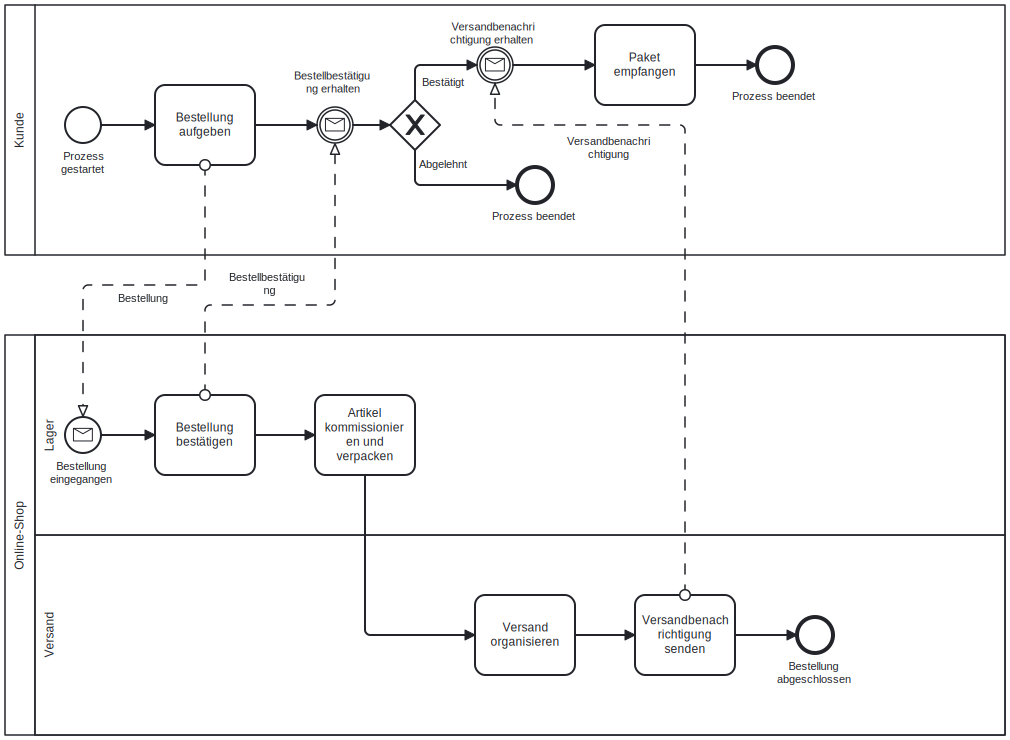
\includegraphics[width=\textwidth]{images/diagrams/diagram_1}
  \caption{Generierung eines Diagrammes}
  \label{fig:detailmode-diagram1}
\end{figure}


Es fällt auf, dass der Bot das Gateway `Ist der Artikel verfügbar' vergessen hat.
Dies ist allerdings kein Problem da das Diagramm nun weiter durch Prompts verbessern kann.
``Bitte bearbeite das Diagramm indem du das vergessene Gateway `Ist der Artikel verfügbar' hinzufügst''
Der Bot erkennt nun wieder, dass keine Textantwort gewünscht ist und beginnt mit der  
Übersendung des neuen Diagramms (\ref{fig:detailmode-diagram2}).

\begin{figure}[ht]
  \centering
  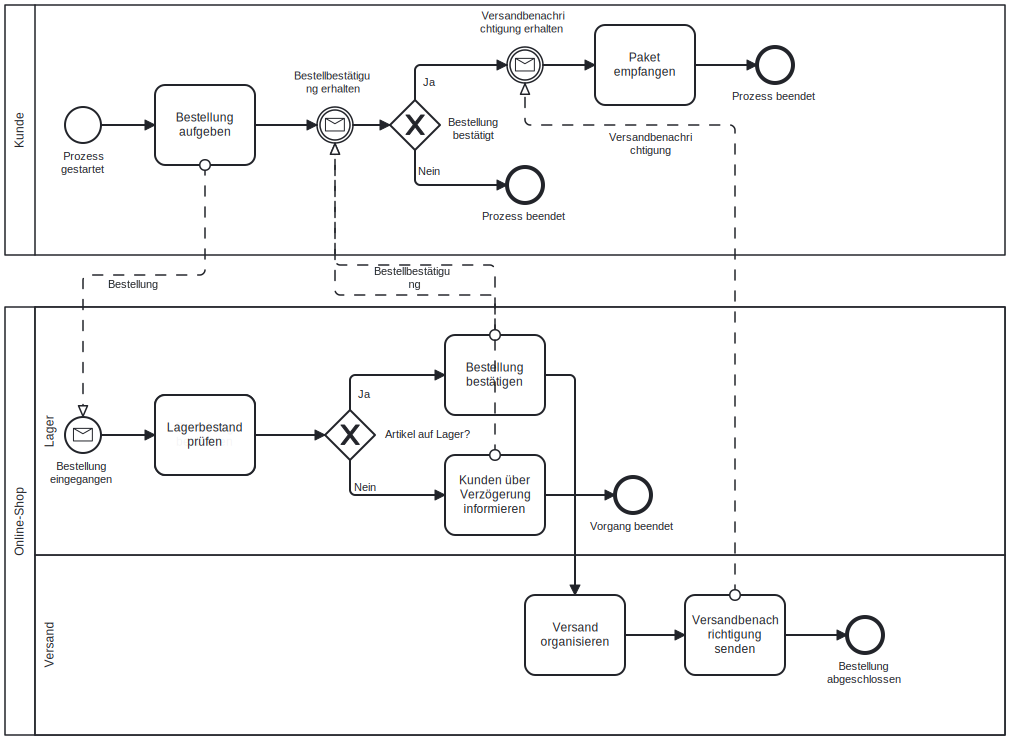
\includegraphics[width=\textwidth]{images/diagrams/diagram_2}
  \caption{Überarbeitung eines Diagrammes mit dem detail mode}
  \label{fig:detailmode-diagram2}
\end{figure}

Das Verhalten des ChatBots entspricht damit exakt den Anforderungen: 
Die Erstellung und Bearbeitung von Diagrammen kann vollständig interaktiv erfolgen, 
und der Nutzer erhält abhängig vom Kontext entweder Klartext oder direkt ein BPMN-Diagramm. 
Im gezeigten Beispiel war die Einordnung der Antwort relativ unkompliziert, 
da jeweils eindeutig erkennbar war, ob die KI ausschließlich Text oder ausschließlich ein 
Diagramm liefern sollte.

Für die weitere Entwicklung soll der Funktionsumfang jedoch erweitert werden, sodass der ChatBot 
künftig auch Antworten erzeugen kann, die Klartext und Diagramm gleichzeitig enthalten. 
Dadurch wird es möglich, dass der Bot zunächst eine Beschreibung, Analyse oder Erklärung liefert 
und anschließend unmittelbar ein dazugehöriges BPMN-Diagramm generiert. 
Ein solcher Anwendungsfall lässt sich beispielsweise mit einer Anfrage wie
„Zeig mir, was du so kannst, indem du eine Prozessbeschreibung erstellst und diese direkt in ein 
Diagramm umsetzt.“
simulieren.

In diesem Szenario entsteht eine neue Herausforderung: 
Die Antwort der KI besteht nicht mehr aus einer einzigen, klaren Kategorie, 
sondern aus zwei unterschiedlichen Inhaltstypen, die voneinander getrennt verarbeitet werden 
müssen. 
Der Klartextteil soll wie gewohnt im Chat ausgegeben werden, während der Diagrammteil in das 
entsprechende Ausgabeformat überführt und anschließend angezeigt wird. 

Zu diesem Zweck wird ein zusätzlicher Erkennungsschritt eingeführt, der die Antwort der KI 
analysiert und die jeweiligen Segmente eindeutig kategorisiert. 
Der ChatBot muss erkennen, welche Abschnitte in natürlicher Sprache formuliert sind und welche 
Bestandteile ein Diagramm darstellen, das weiterverarbeitet werden soll. 
Dieses Verhalten ermöglicht eine deutlich flexiblere Interaktion und ermöglicht neue 
Möglichkeiten, besonders dann, wenn der Nutzer sowohl inhaltliche Erläuterungen als auch die 
direkte Umsetzung in ein BPMN-Diagramm erwartet.

Für dieses Kategorisierung wird eine Beispiel-Antwort betrachtet, welche hier zum Verständnis nicht
per Markdown formatiert ist:

\noindent\fbox{
  \parbox{.96\textwidth}{
    Gerne, hier ist ein Vorschlag für einen einfachen, aber vollständigen Prozess: \\
    **Prozess:** Urlaubsantrag **Beteiligte:** Mitarbeiter, Vorgesetzter \\
    **Ablauf:** 1. Ein Mitarbeiter füllt einen Urlaubsantrag aus und reicht ihn ein. \\
    2. Der Vorgesetzte erhält den Antrag und prüft ihn. \\
    3. Der Vorgesetzte entscheidet, ob der Antrag genehmigt oder abgelehnt wird. \\
    * **Bei Genehmigung:** Der Mitarbeiter wird über die Genehmigung informiert. \\
    * **Bei Ablehnung:** Der Mitarbeiter wird über die Ablehnung informiert. \\
    4. Der Prozess ist in beiden Fällen abgeschlossen. \\
    \colorbox{black!0}{\strut\textasciigrave\textasciigrave\textasciigrave xml}%
    \colorbox{black!0}{\strut<?xml version=1.0 encoding=UTF-8?><bpmn:definitions}\\
    \colorbox{black!0}{\parbox{\linewidth-10pt}{\strut[\ldots]}}\\
    \colorbox{black!0}{\strut</bpmn:definitions>}%
    \colorbox{black!0}{\strut\textasciigrave\textasciigrave\textasciigrave}\\
    In diesem Beispiel gibt es ein \\ 
    \colorbox{black!0}{\strut<bpmn:startEvent name=``Urlaubsantrag ausgefüllt''>}, ein \\
    \colorbox{black!0}{\strut\textasciigrave}%
    \colorbox{black!0}{\strut<bpmn:exclusiveGateway name=``Antrag genehmigt''>}%
    \colorbox{black!0}{\strut\textasciigrave}
    und weitere tasks welche den Ablauf eines Urlaubsantrags zeigen.
  }
}

Der Algorithmus soll nun zunächst alle Diagramme finden.
Dies wird hier durch den Aufruf eines Regex ermöglicht.
Das Regex ist in Abbildung~\ref{code:regex} zu sehen.

\begin{code}
\begin{minted}[frame=single, framesep=2pt, linenos, fontsize=\small, style=vs, breaklines, breakanywhere]{typescript}
/(?:``?`?\s*(?:xml)?\s*)?(<[^<>]*\/[^<>]*>\s*|<[^\/<>]*>[^`]*<\/[^<>]*>)+\s*(?:``?`?|(?=[^<>`\s]))\n?/g
\end{minted}
\caption{Regex zur Diagrammerkennung}
\label{code:regex}
\end{code}

Über dieses werden automatisch alle validen XML Teile (Im folgenden Beispiel bunt markiert) erkannt.
Durch die Benutzung einer Non-capturing-group werden Wrapper des XML 
(Im folgenden Beispiel dunkelblau markiert) wie zum Beispiel das 
`\textasciigrave\textasciigrave\textasciigrave xml', automatisch entfernt.
Alle gefundenen Übereinstimmungen werden danach auf ihre Länge geprüft um herauszufinden ob diese ein 
vollständiges Diagramm repräsentieren oder nur eine Referenz bzw. Erklärung als 
Teil des Klartextes sind. (Im folgenden Beispiel gelb markiert)

\noindent\fbox{
  \parbox{.96\textwidth}{
    Gerne, hier ist ein Vorschlag für einen einfachen, aber vollständigen Prozess: \\
    **Prozess:** Urlaubsantrag **Beteiligte:** Mitarbeiter, Vorgesetzter \\
    **Ablauf:** 1. Ein Mitarbeiter füllt einen Urlaubsantrag aus und reicht ihn ein. \\
    2. Der Vorgesetzte erhält den Antrag und prüft ihn. \\
    3. Der Vorgesetzte entscheidet, ob der Antrag genehmigt oder abgelehnt wird. \\
    * **Bei Genehmigung:** Der Mitarbeiter wird über die Genehmigung informiert. \\
    * **Bei Ablehnung:** Der Mitarbeiter wird über die Ablehnung informiert. \\
    4. Der Prozess ist in beiden Fällen abgeschlossen. \\
    \colorbox{blue!60}{\strut\textasciigrave\textasciigrave\textasciigrave xml}%
    \colorbox{cyan!60}{\parbox{\linewidth-48pt}{\strut<?xml version=1.0 encoding=UTF-8?><bpmn:definitions}}\\
    \colorbox{cyan!60}{\parbox{\linewidth-7pt}{\strut[\ldots]}}\\
    \colorbox{cyan!60}{\strut</bpmn:definitions>}%
    \colorbox{blue!60}{\strut\textasciigrave\textasciigrave\textasciigrave}
    In diesem Beispiel gibt es ein \\ 
    \colorbox{yellow!60}{\strut<bpmn:startEvent name=``Urlaubsantrag ausgefüllt''>}, ein \\
    \colorbox{blue!60}{\strut\textasciigrave}%
    \colorbox{yellow!60}{\strut<bpmn:exclusiveGateway name=``Antrag genehmigt''>}%
    \colorbox{blue!60}{\strut\textasciigrave}
    und weitere tasks welche den Ablauf eines Urlaubsantrags zeigen.
  }
}

Somit kann die gesamte Nachricht kategorisiert werden.
Hellblaue Textstellen sind Diagramme,
Nicht markierte Teile und gelbe Textstellen sind Teil der Klartextnachricht.

So wie hier für eine Nachricht mit XML-Diagrammen kann auch eine Nachricht konzeptgleich mit JSON-Diagrammen 
kategorisiert werden.

\section{Weitere Anbieter}

Es ist sinnvoll, dass der Chatbot neben ChatGPT auch andere Chatbot-Anbieter 
nutzen kann, um Flexibilität, Ausfallsicherheit und Vielfalt in den 
Antwortmöglichkeiten sicherzustellen. 
Unterschiedliche Anbieter bieten verschiedene Stärken, wie etwa spezialisierte Natural 
Language Processing-Modelle, schnellere Antwortzeiten oder kosteneffizientere Lösungen. 
Durch die Integration mehrerer Anbieter kann je nach Bedarf die beste Leistung ausgewählt werden 
und Ausfälle eines einzelnen Dienstes werden abgefedert. 
Dies erhöht die Zuverlässigkeit und Qualität der generierten BPMN-Diagramme.

Durch die objektorientierte Konfiguration der KI Schnittstelle ist es zudem sehr einfach weitere 
Anbieter hinzuzufügen.

\subsection{Grok}

Die Einbindung von Grok ergänzt ChatGPT, weil Grok schneller auf aktuelle Daten zugreift, oft 
direkter formuliert und technische Zusammenhänge sehr präzise erkennt. 
Dadurch kann der Bot bei bestimmten Aufgaben, etwa beim Interpretieren knapper Anweisungen 
oder beim Erzeugen alternativer BPMN-Varianten, Ergebnisse liefern, die ChatGPT allein nicht 
immer erreicht. 

Grok kann einfach über die XAI SDK 
\footnote{\url{https://ai-sdk.dev/providers/ai-sdk-providers/xai}}
und die Typescript AI SDK
\footnote{\url{https://www.npmjs.com/package/ai}}
zu BPMN-Gen hinzugefügt werden.

Hierfür wird eine Klasse Grok erstellt, welche die Ai Klasse vererbt bekommt und damit nur 
noch die Schnittstelle der Grok API implementieren muss.
Der entscheidende Schritt ist hierbei die zu versendende Nachricht an die Grok API vom PromptInput Objekt auf das 
API Format zu bringen.
Diese Konvertierung kann man in Codeauschnitt~\ref{code:grok-format} sehen.

Folgende Modelle sind damit zum aktuellen Stand für BPMN-Gen verfügbar:

\begin{table}[h!]
  \centering
  \begin{tabular}{lrr}
      \toprule
      Model & Input-Kosten & Output-Kosten \\
      \midrule
      grok-4-1-fast-reasoning & 0.20 \$ & 0.50 \$ \\
      grok-4-fast-reasoning & 0.20 \$ & 0.50 \$ \\
      grok-4-1-fast-non-reasoning & 0.20 \$ & 0.50 \$ \\
      grok-4-fast-non-reasoning & 0.20 \$ & 0.50 \$ \\
      grok-code-fast-1 & 0.20 \$ & 1.50 \$ \\
      grok-4 & 3.00 \$ & 15.00 \$ \\
      grok-3-mini & 0.30 \$ & 0.50 \$ \\
      grok-3 & 3.00 \$ & 15.00 \$ \\
      \bottomrule
  \end{tabular}
  \caption{Modelle von xAI \\ (Stand: 20.11.2025)}
  \label{tab:grok-models}
\end{table}

\begin{code}[H]
\begin{minted}[frame=single, framesep=2pt, linenos, fontsize=\small, style=vs]{typescript}
protected mapPromptInput(input: PromptInput) {
  const historyInst = input.history.map((item) => {
    return {role: item.role, content: item.content} ;
  })
  const fileInst = input.file ? {
    role: "user",
    content: [{
      type: "image",
      image: input.getFileDataUrl() ,
    }],
  } : [];
  const userInst = {role: "user", content: input.prompt}
  return {
    model: this.xai(this.model),
    system: input.instructions.join("\n"),
    messages: [historyInst, userInst, fileInst],
  };
}
\end{minted}
\caption{mapPromptInput() für Grok}
\label{code:grok-format}
\end{code}

Die Nachricht wird dann mit Hilfe der AI SDK an Grok gesendet und die Antwort empfangen.

\subsection{Gemini}

Die Einbindung von Gemini ergänzt ChatGPT, weil Gemini bei komplexen Analyseaufgaben, 
strukturiertem Denken und dem Umgang mit großen Informationsmengen besonders stark ist. 
Dadurch kann der Bot bei der Modellierung und Optimierung von BPMN-Prozessen zusätzliche 
Präzision und alternative Lösungswege bieten. Gemini erhöht so die fachliche Tiefe, Robustheit 
und Variantenvielfalt der Ergebnisse.
Gemini hat zum aktuellen Zeitpunkt auch einen entscheidenden Vorteil gegenüber den anderen 
LLM Anbietern.
Die API hat auch eine kostenlose Stufe, wodurch es möglich ist, bis zu einer gewissen 
Menge an Anfragen, Diagramme zu erstellen, welche kein Geld kosten.

Ähnlich wie bei Grok wird nun die Klasse Gemini erstellt, welche die Schnittstelle zur API
implementiert.
Dies passiert über die Gemini SDK
\footnote{\url{https://ai.google.dev/gemini-api/docs?hl=de}},
für welche die Anfrage wieder auf das gewünschte Format gebracht werden muss.

Durch Gemeini sind dannn diese Modelle alle benutzbar:

\begin{table}[h!]
  \centering
  \begin{tabular}{lrr}
      \toprule
      Model & Input-Kosten & Output-Kosten \\
      \midrule
      gemini-2.5-pro & 0.00 \$ & 0.00 \$ \\
      gemini-2.5-flash & 0.00 \$ & 0.00 \$ \\
      gemini-2.5-flash-lite & 0.00 \$ & 0.00 \$ \\
      gemini-2.0-flash & 0.00 \$ & 0.00 \$ \\
      \midrule
      \multicolumn{3}{l}{Nicht auf der kostelosen Stufe verfügbar:} \\
      gemini-3-pro-preview & 2.00 \$ & 12.00 \$ \\
      \bottomrule
  \end{tabular}
  \caption{Modelle von Google \\ (Stand: 20.11.2025)}
  \label{tab:gemini-models}
\end{table}


\begin{code}[H]
\begin{minted}[frame=single, framesep=2pt, linenos, fontsize=\small, style=vs]{typescript}
protected mapPromptInput(input: PromptInput) {
  const systemInst = input.instructions.map((instruction) => {
    return {
      role: "model", 
      parts: [{text: instruction, thought: false}]
    };
  });
  const historyInst = input.history.map((item) => {
    return {
      role: item.role == "user" ? "user" : "model",
      parts: [{
        text: item.content, 
        thought: item.role == "assistant"
      }],
    };
  });
  const imageInst = input.file ? {
    role: "user", parts: [{
      type: "input_file",
      inlineData: {
        data: input.getFileBase64Data(),
        mimeType: input.getFileMimeType(),
      },
    }]} : [];
  const userInst = {
    role: "user", 
    parts: [{text: input.prompt}]
  };
  return {
    model: this.model,
    contents: [systemInst, historyInst, userInst, imageInst],
  };
}
\end{minted}
\caption{mapPromptInput() für Gemini}
\label{code:gemini-format}
\end{code}

Die Gemini API erwartet bei Jedem Textteil der Anfrage noch das Feld `thought', welches angibt
ob dieser Teil bereit von einer KI gedacht wurde.

\subsection{Claude}

Claude ergänzt BPMN-Gen besonders gut, weil er stark auf programmierbezogene Aufgaben 
spezialisiert ist. 
Sein Modell ist darauf ausgelegt, Code sehr zuverlässig zu verstehen, zu strukturieren und 
zu korrigieren. 
Dadurch liefert Claude bei der Umsetzung von BPMN-Diagrammen in JSON und XML
und bei der Fehleranalyse oft besonders saubere Ergebnisse, da diese Formate besonders
gut verstanden und umgesetzt werden.
Die Einbindung von Claude erhöht somit die Präzision und Qualität von
BPMN-Gen.

Claude wird nun wie schon bei den anderen Anietern über seine eigene Klasse zu BPMN-Gen 
hinzugefügt. Hierbei wird die Schnittstelle, wie in Codeausschnitt~\ref{code:claude-format},
über die Anthropic SDK implemenitert.
\footnote{\url{https://platform.claude.com/docs/en/api/client-sdks}}

Mit Claude sind dann auch noch diese Modelle verfügbar:

\begin{table}[h!]
  \centering
  \begin{tabular}{lrr}
      \toprule
      Model & Input-Kosten & Output-Kosten \\
      \midrule
      claude-opus-4-5 & 5.00 \$ & 25.00 \$ \\
      claude-opus-4-1 & 15.00 \$ & 75.00 \$ \\
      claude-sonnet-4-5 & 3.00 \$ & 15.00 \$ \\
      claude-haiku-4-5 & 1.00 \$ & 5.00 \$ \\
      claude-sonnet-4 & 3.00 \$ & 15.00 \$ \\
      claude-opus-4 & 15.00 \$ & 75.00 \$ \\
      claude-sonnet-3-7 & 3.00 \$ & 15.00 \$ \\
      claude-haiku-3-5 & 0.80 \$ & 4.00 \$ \\
      claude-opus-3 & 15.00 \$ & 75.00 \$ \\
      \bottomrule
  \end{tabular}
  \caption{Modelle von Anthropic \\ (Stand: 20.11.2025)}
  \label{tab:claude-modelle}
\end{table}

\begin{code}[H]
\begin{minted}[frame=single, framesep=2pt, linenos, fontsize=\small, style=vs]{typescript}
protected mapPromptInput(input: PromptInput) {
  const systemInst = input.instructions.map((instruction) => {
    return {type: "text", text: instruction};
  });
  const historyInst = input.history.map((item) => {
    return {role: item.role, content: item.content};
  });
  const imageInst = input.file ? {
    role: "user",
    content: [{
      type: "file",
      source: {
        type: 'base64',
        data: input.getFileBase64Data(),
        media_type: input.getFileMimeType(),
      },
    }],
  } : [];
  const userInst = {role: "user", content: input.prompt};
  return {
    model: this.model,
    max_tokens: 15000,
    system: systemInst,
    messages: [historyInst, userInst, imageInst],
  };
}
\end{minted}
\caption{mapPromptInput() für Claude}
\label{code:claude-format}
\end{code}

\section{Streaming}

Bisher ergab es nur begrenzt Sinn, die Antworten der KI zu streamen, da ein Diagramm erst dann 
nutzbar ist, wenn es vollständig erzeugt wurde. 
Einzelne, unvollständige Fragmente eines BPMN-Diagramms bieten keinen Mehrwert und können vom 
Client nicht sinnvoll verarbeitet oder angezeigt werden. 
Mit der Einführung gemischter Antworten, die sowohl Klartext als auch Diagramme enthalten können, 
ändert sich dies jedoch.

Sobald ein Teil der Antwort aus natürlicher Sprache besteht, entsteht ein klarer Vorteil beim 
Streaming. 
Textinhalte können bereits angezeigt werden, während der restliche Output noch generiert wird. 
Dadurch erhält der Nutzer deutlich schneller Rückmeldung, was insbesondere bei komplexeren oder 
längeren Antworten zu einem spürbar verbesserten Nutzungserlebnis führt.

Technisch bedeutet dies, dass die Ausgabe der KI zunächst an den BPMNGen-Server gestreamt werden 
muss, der die eingehenden Daten analysiert und korrekt kategorisiert. 
Anschließend wird der Klartext Teil der Antwort weiter an den Client gestreamt. 
Entscheidend ist dabei, dass ausschließlich der textuelle Anteil der Antwort übertragen wird. 
Diagrammfragmente oder Codeblöcke würden beim Client zu Fehlern führen, da diese erst nach 
vollständiger Generierung sinnvoll weiterverarbeitet oder angezeigt werden können.

Durch diese Trennung entsteht ein effizientes zweistufiges Streaming-Verfahren: 
Der BPMNGen-Server verarbeitet die gesamte Antwort, extrahiert den Klartext in Echtzeit und 
leitet ihn unmittelbar weiter, während das Diagramm erst nach seiner vollständigen Fertigstellung 
bereitgestellt wird. 

Die gestreamte Ausgabe eines LLM-Anbieters zu starten ist in den meisten Fällen unkompliziert. 
Viele Modelle bieten dafür einen expliziten Parameter an, der direkt in der Anfrage gesetzt 
werden kann. 
Sowohl ChatGPT als auch Claude unterstützen dieses Vorgehen nativ, sodass sich das gewünschte 
Verhalten bereits beim Abschicken des Requests konfigurieren lässt. 
Ein entsprechendes Beispiel sieht wie folgt aus:

\begin{code}
\begin{minted}[frame=single, framesep=2pt, linenos, fontsize=\small, style=vs]{typescript}
protected mapPromptInput(input: PromptInput, stream: boolean) {
  [...]
  return {
    model: this.model,
    stream: stream,
    system: systemInst,
    input: [historyInst, userInst, imageInst]
  };
}
\end{minted}
\caption{mapPromptInput() für einen Stream}
\label{code:chatgpt-format-stream}
\end{code}

Andere Anbieter wie Gemini oder Grok verfolgen dagegen einen leicht unterschiedlichen Ansatz und 
stellen das Streaming über eine separate API-Funktion bereit. 
Je nach verwendetem Endpunkt wird entweder ein normaler Text generiert oder ein Stream 
zurückgegeben. 
Der Wechsel zwischen beiden Varianten lässt sich dadurch einfach implementieren:

\begin{code}
\begin{minted}[frame=single, framesep=2pt, linenos, fontsize=\small, style=vs]{typescript}
async generateContent(input: any, stream: boolean) {
  if (stream) return streamText(input)
  return generateText(input);
}
\end{minted}
\caption{generateContent() für einen Stream}
\label{code:grok-format-stream}
\end{code}

Sobald die Antwort der KI eintrifft, wird zunächst überprüft, ob es sich tatsächlich um einen 
Stream handelt. 
Da JavaScript-basierte Streams typischerweise das Symbol \texttt{asyncIterator} implementieren, 
lässt sich dies zuverlässig über eine einfache Typprüfung feststellen:

\begin{code}
\begin{minted}[frame=single, framesep=2pt, linenos, fontsize=\small, style=vs]{typescript}
protected isStream(obj: any): boolean {
  return obj && typeof obj[Symbol.asyncIterator] == "function";
}
\end{minted}
\caption{isStream()}
\label{code:is-stream}
\end{code}

Wird ein Stream erkannt, kann dieser anschließend mithilfe eines asynchronen Iterations-Loops 
ausgelesen werden. 
Die empfangenen Delta-Fragmente lassen sich so in Echtzeit weiterverarbeiten, um 
Klartext sofort an den Client zu streamen, bevor das vollständige Diagramm erzeugt wird.

\begin{code}
\begin{minted}[frame=single, framesep=2pt, linenos, fontsize=\small, style=vs]{typescript}
protected async processStream(stream: any){
  for await (const chunk of stream) {
    switch (chunk.type) {
      case "response.output_text.delta":
        // Text oder andere Änderungen
        processDelta(chunk.delta);
        break;

      case "response.completed":
        // Fertig gelesen
        return;

      case "response.error":
      case "response.failed":
        // Fehler
        error(chunk.response.error.message);
        return;

      default:
        break;
    }
  }
}
\end{minted}
\caption{processStream()}
\label{code:process-stream}
\end{code}

Während der Stream verarbeitet wird, wird die Antwort der KI schrittweise in einem internen 
Buffer aufgebaut. 
Nach jeder Erweiterung des Buffers wird der Klartextanteil, wie in Abschnitt~\ref{sec:konversationen}
beschrieben, extrahiert und an den Client weitergeleitet. 
Auf diese Weise erhält der Nutzer bereits während der Generierung der vollständigen Antwort 
fortlaufend Informationen, ohne auf das Endergebnis warten zu müssen.

Erkennt das System jedoch, dass der Stream aktuell ein Diagramm enthält, wird dieser 
zunächst zurückgehalten und nicht an den Client übertragen. 
Diagrammfragmente sind während der laufenden Generierung weder syntaktisch vollständig noch 
anzeigbar. 
Es macht daher keinen Sinn diese zu streamen.

Sobald das Diagramm allerdings vollständig empfangen wurde, kann es analysiert und eindeutig 
einer Kategorie zugeordnet werden. 
Dabei wird, wie in Abschnitt~\ref{sec:konversationen} beschrieben, entschieden, ob es sich um ein 
finales BPMN-Diagramm handelt, das angezeigt werden soll, oder ob der betreffende Abschnitt 
lediglich Bestandteil eines beschreibenden Klartextes ist und somit kein eigenständiges 
Diagramm ist. 
Dieses Vorgehen stellt sicher, dass sowohl Text- als auch Diagrammausgaben sauber voneinander 
getrennt und jeweils korrekt verarbeitet werden, ohne dass unvollständige oder fehlerhafte 
Diagrammfragmente beim Client ankommen.

\subsection{SSE}

Für die Übertragung der erzeugten Informationen an den Client wird die Technik der Server-Sent 
Events (SSE) eingesetzt. 
SSE ermöglicht es dem Server, Daten in Echtzeit an den Client zu senden, ohne dass dieser 
wiederholt aktiv Anfragen stellen muss. 
Jede gesendete Nachricht folgt dabei einem strukturierten Aufbau und besteht aus zwei 
wesentlichen Komponenten: einem \texttt{event}-Feld und einem \texttt{data}-Feld.

Der \texttt{event}-Teil enthält in der Regel ein einzelnes Wort, das den Typ oder die Bedeutung 
der übertragenen Daten beschreibt, zum Beispiel \texttt{delta}, \texttt{diagram}, \texttt{error} 
oder \texttt{end}. 
Dadurch kann der Client umgehend erkennen, wie der empfangene Inhalt weiterzuverarbeiten ist.

Der eigentliche Inhalt befindet sich im \texttt{data}-Teil. 
Hier werden die Daten hinterlegt, beispielsweise ein Textdelta oder ein fertig generiertes 
Diagramm.

Zusammengefügt und korrekt formatiert wird die gesamte SSE-Nachricht schließlich in folgender 
Form an den Client übermittelt:

\noindent\fbox{
  \parbox{.96\textwidth}{
    event: \textit{event-name}\\
    data: \textit{Erste Zeile der Daten}\\
    data: \textit{Weitere Zeile mit Daten}\\

    event: \textit{Nächstes Event}\\
    \ldots
  }
}

Im folgenden wird nun gezeigt welche Events für die Übertragung einer Antwort an den Client
implementiert wurden.

Der Stream beginnt mit einem \texttt{start} Event. In diesem wird dem Client die Thread-ID mitgeteilt
und indirekt erkenntlich gemacht, dass nun ein Stream gestartet wird.

Da manche KI Anbieter Modelle entwickelt haben, welche zunächst Websuchen durchführen oder interne 
Prozesse durchführen,
kann es sein, dass zwischen dem Start des Streams und dem ersten Delta einiges an Zeit vergeht.
Um zu verhindern, dass der Browser des Clients deshalb durch einen Timeout die Verbindung schliesst,
wird das \texttt{alive} Event implementiert.
Dieses wird jede Sekunde gesendet und beinhaltet als data jedeglich die aktuelle Uhrzeit.

Das erste eigentliche Daten Event ist nun das \texttt{delta} Event bis dem die tatsächlichen
Deltas des Klartextteils versendet werden. 
Die Deltas haben keine fixe größe und können je nach LLM Anbieter und Antwort variieren.

Jegliche Fehler werden dem Client als \texttt{error} Event mitgleteil, wobei die Error Nachricht
als Data mitgesendet wird. Nach einem \texttt{error} Event wird die Verbindung automatisch vom 
Server beendet.

Wenn der Server erkennt, dass gerade ein vollständiges Diagramm generiert wird, sendet er ein
\texttt{diagram-start} Event welches dem Client mitteilt, welches Modell verwendet wird.
Sobald das Diagramm fertig generiert wurde, wird auch ein \texttt{diagram-end} Event gesendet,
welches dem Client mitteilt, dass das Diagramm fertig erzeugt wurde,
sowie ein \texttt{diagram} Event, welches das fertige und formatierte Diagramm enthält.

Sobald der Stream des LLMs fertig ist, wird noch ein \texttt{end} Event versendet, welches die
gesamte Antwort als JSON versendet, genau so, wie die Antwort gewesen wäre, falls nicht an
den Client gestreamt worden wäre. Dies ist da um mögliche Fehler bei der Übersendung des Streams
ausbessern zu können.

Final wird noch ein \texttt{save} Event versendet, welches dem Client mitteilt, dass die generierte
Antwort nun auch erfolgreich in der Datenbank abgespeichert wurde und nun für weitere Anfragen 
bereit steht.
Danach wird der Stream geschlossen und die Übertragung ist abgeschlossen.

\noindent\fbox{
  \parbox{.96\textwidth}{
    event: start\\
    data: faf8ad85-5546-4da2-98d9-8784844f1ea9\\
    
    event: delta\\
    data: Ich bin\\

    event: delta\\
    data: ChatGPT 4.1 mini\\

    event: diagram-start\\
    data: gpt-4.1-mini\\

    event: alive\\
    data: 01.01.2025 00:02\\

    event: diagram-end\\
    data: gpt-4.1-mini\\

    event: diagram\\
    data: <?xml version=\textbackslash``1.0\textbackslash'' encoding=\textbackslash``UTF-8\textbackslash''?>\\
    data: <bpmn:definitions \ldots\\
    data: </bpmn:definitions>\\

    event: end\\
    data: \{ \\
    data: ``text'': ``Ich bin ChatGPT 4.1 mini''\\
    data: ``xml'': ``<?xml?><bpmn:definitions>\ldots</bpmn:definitions>''\\
    data: \}\\
    
    event: save\\
    data: success\\
  }
}

\section{Schema-Constraining}

Schema Constraining bezeichnet die Technik, bei der das Ausgabeformat eines KI-Modells 
durch ein vorgegebenes Schema eingeschränkt wird. 
Statt den Text frei formulieren zu können, muss das Modell seine Antwort exakt in der 
festgelegten Struktur ausgeben.
Dies kann beispielsweise ein JSON-Schema, ein XML-Schema oder eine 
andere Form haben. 
Schema Constraing wurde bereits auch bei vergleichbaren BPMN Bots eingesetzt
und hat erfolgreich alle syntaktischen Fehler eliminieren können.
~\cite{koeppke2025BPMNChatbotPP} 

Der große Vorteil besteht darin, dass die Antworten vorhersehbar sind. 
Fehler wie fehlende Felder, falsche Datentypen oder ungültige Strukturen werden 
verhindert, da das Modell gezwungen ist, jede Ausgabe formal korrekt zu gestalten. 
Dies ist besonders wichtig in Anwendungen, bei denen die KI-Ausgabe 
weiterverarbeitet wird, wie etwa bei der Erstellung von 
BPMN-Diagrammen.

Dadurch ist sichergestellt, dass alle erzeugten Diagramme syntaktisch korrekt sind.
Allerdings kann das Schema-Constraining nicht auf den \texttt{detail} Modus 
angewendet werden, da dieser nach dem Design auch frei mit Klartext, Beschreibungen,
Beispielen, Fragen und allem was gewünscht wird antworten können soll.
Daher wird das Schema Constraining bei dem \texttt{quick} Modus verwendet.

Die Nutzung des Schema Constraining wird von allen Anbietern bereitgestellt, allerdings  
hat auch jeder Anbieter seine eigene Umsetztung dieser Constraints.
Alle Anbieter erlauben aber die Nutzung des Schema-Validators \texttt{zod}.
\footnote{\url{https://zod.dev/}}
Hierbei wird das Schema über Objects, Arrays und Enums abbilden, wobei diese jeweils
primitive Attribute besitzen wie z.B.\@ numbers, strings, booleans, uuids, chars\dots

Mit zod lässt sich sehr gut das definierte JSON Schema darstellen.
Wie diese Schema Constraints für JSON aussehen, wird in Codeausschnitt~\ref{code:schema}
gezeigt.
Eine Unterstützung für XML Schemas ist leider mit Zod nur begrenzt möglich.

\begin{code}
\begin{minted}[frame=single, framesep=2pt, linenos, fontsize=\footnotesize, style=vs]{typescript}
const CoordinateSchema = z.array(
  z.number().int().nonnegative()
).length(2);
const ComponentTypeEnum = z.enum([
  'startEvent','messageStartEvent','timerStartEvent',
  'intermediateCatchEvent','intermediateThrowEvent',
  'messageCatchEvent','messageThrowEvent','timerIntermediateEvent',
  'endEvent','messageEndEvent','task','subProcess',
  'exclusiveGateway','parallelGateway','inclusiveGateway'
]);
const FlowTypeEnum = z.enum([
  'sequenceFlow','messageFlow','association',
  'dataInputAssociation','dataOutputAssociation',
]);
const FlowSchema = z.object({
  ID: z.string().min(1),
  Start: z.string(),
  Target: z.string(),
  Type: FlowTypeEnum,
  StartXY: CoordinateSchema,
  TargetXY: CoordinateSchema,
  Descriptor: z.string(),
});
const ComponentSchema: z.ZodType<any> = z.lazy(() => z.object({
    ID: z.string().min(1),
    Name: z.string(),
    Type: ComponentTypeEnum,
    x: z.number().int().nonnegative(),
    y: z.number().int().nonnegative(),
    Incoming: z.array(z.string()),
    Outgoing: z.array(z.string()),
    Components: z.array(ComponentSchema).optional().nullable(),
    Flows: z.array(FlowSchema).optional().nullable(),
}));
const LaneSchema = z.object({
  ID: z.string().min(1),
  Name: z.string().min(1),
  XY: CoordinateSchema,
  width: z.number().int().positive(),
  height: z.number().int().positive(),
  Components: z.array(ComponentSchema),
  Flows: z.array(FlowSchema),
});
\end{minted}
\caption{Schema Constraining with ZOD}
\label{code:schema}
\end{code}

\section{Diagramm-Sampling}

Während die Bezeichnung \texttt{Spampling} in Bezug auf LLMs bereits eine Bedeutung
hat, wird hier im Bezug auf BPMN Generierung nicht von Token-Sampling sondern von
Diagramm-Sampling gesprochen.

Der Begriff „Sampling“ bedeutet im Kontext von KI-Modellen allgemein: 
``Aus einer Menge möglicher Modellantworten mehrere Alternativen erzeugen''

Dies bedeutet konkret, dass beim Token-Sampling mehrere Token erstellt werden und
daraus das beste gewählt wird.
Beim Sampling für Diagramme werden nun auch mehrere Diagramme erstellt.
Allerdings ist es schwierig zu beurteilen, welches Diagramm nun das `beste' ist.
Darum werden bei der erstellung der Diagramme klar festgelegt, welche Anbieter 
ein Diagramm erzeugen und alle werden dem Nutzer präsentiert, da dieser selber 
am besten die Qualität beurteilen kann.

Die Erstellung mehrerer Diagramme erfolgt, indem die selbe textuelle 
Prozessbeschreibung parallel an verschiedene Sprachmodelle bzw. KI-Anbieter 
gesendet wird. 
Jedes Modell generiert daraufhin ein vollständiges BPMN-Diagramm, 
basierend auf seiner internen Architektur und Trainingsdaten. 
Durch den gleichen Prompt wird 
sichergestellt, dass alle Modelle unter vergleichbaren Bedingungen arbeiten und 
somit miteinander vergleichbare Ergebnisse liefern. 
Dieser parallele Erstellungsprozess ermöglicht es, innerhalb eines einzigen 
Ausführungsvorgangs mehrere unabhängige Modellierungen desselben Prozesses zu 
erhalten, ohne zusätzliche Laufzeit oder iterative Interaktion mit einem einzelnen 
Modell zu benötigen. 

Da keine zusätzlichen textuellen Ausgaben benötigt werden, erfolgt die Generierung 
der zusätzlichen Diagramme ausschließlich im \texttt{quick}-Modus. 
Die Auswahl der Modelle, die für die parallele Diagrammerzeugung genutzt werden, 
ist flexibel und kann vom Nutzer oder vom Client als Parameter 
der Anfrage frei bestimmt werden. 
Dadurch lässt sich die Zahl der beteiligten Anbieter dynamisch variieren, was 
insbesondere für Vergleiche oder Qualitätssicherung von 
Vorteil ist.

Alle erzeugten Diagramme, unabhängig davon, welches Modell sie generiert hat, 
werden anschließend gesammelt und gebündelt an den Client übermittelt. 
Dies ermöglicht es, die Ergebnisse unmittelbar nebeneinander anzuzeigen, 
wodurch der Nutzer einen direkten Vergleich der unterschiedlichen 
Modelle erhält. 

Eine Anfrage mit Diagramm Sampling kann in etwa so aussehen wie in Anfrage 
~\ref{code:post-samples}.

\begin{code}
\begin{minted}[frame=single, framesep=2pt, linenos, fontsize=\small, style=vs]{json}
// POST /threads
{ 
  "inputString": "Bitte generiere mir ein BPMN Diagram, 
      welches den Ablauf in einem Restaurant zeigt", 
  "model": "gpt-5 (xml)",
  "mode": "detail",
  "samples": [
    "gemini-2.5-pro (xml)",
    "grok-4 (json)"
  ]
}
\end{minted}
\caption{Post Request an /threads mit Sampling}
\label{code:post-samples}
\end{code}

Der Code in Codeausschnitt~\ref{code:run-samples} führt die parallele Generierung 
aller BPMN-Diagramme aus. 
Zunächst wird anhand des ausgewählten Modells die primäre Genereierung vorbereitet.
Die Sampling-Modelle, hier die sekundären genannt, werden zunächst gefiltert, um 
ungültige Einträge sowie Duplikate zu 
entfernen, und anschließend auf maximal fünf zusätzliche Modelle begrenzt. 
Für jedes dieser Modelle wird ebenfalls die Diagrammgenerierung vorbereitet, jedoch im 
ressourcenschonenden \texttt{quick}-Modus.

Alle Diagramm-Generierungen, das primäre sowie die sekundären, werden schließlich 
über \mintinline{typescript}{Promise.all([])} parallel ausgeführt. 
Dadurch entstehen mehrere unabhängige Modellantworten in einem einzigen 
Ausführungsschritt, die anschließend gemeinsam an den Client geschickt werden.

\begin{code}
\begin{minted}[frame=single, framesep=2pt, linenos, fontsize=\small, style=vs]{typescript}
const gpt = getGPT(model, format)!;
const sampling = !!samples;
const primary = gpt.createBPMN([...], mode, "primary");
const secondaries = samples
  .map(str => getGPT(str))
  .filter(gpt => !!gpt)                   // remove invalid
  .filter((v, i, s) => s.indexOf(v) == i) // remove duplicates
  .slice(0, 5)                            // limit to 5 samples
  .map(gpt => gpt.createBPMN([...], "quick", "secondary"));
const outputs = await Promise.all([primary, ...secondaries]);
\end{minted}
\caption{Ausführung der Samples}
\label{code:run-samples}
\end{code}

\section{Reflective Prompting}

Reflective Prompting ist eine Technik, bei der ein KI-Modell bewusst dazu angeleitet wird, über 
seine eigenen Antworten nachzudenken, bevor es ein endgültiges Ergebnis liefert. 
Anders als beim klassischen Prompting, bei dem das Modell direkt versucht, die bestmögliche 
Antwort zu erzeugen, besteht Reflective Prompting aus zwei Stufen: 
Zuerst erstellt das Modell einen Entwurf oder eine Einschätzung, anschließend überprüft es diesen 
Entwurf selbstständig, reflektiert mögliche Fehler oder Unklarheiten und verbessert die Antwort 
basierend auf dieser Selbstkritik.

Dieses Vorgehen hat mehrere Vorteile. 
Das Modell erkennt häufiger eigene Ungenauigkeiten, identifiziert logische Fehler oder fehlende 
Details und kann dadurch qualitativ hochwertigere Ergebnisse liefern. 
Reflective Prompting eignet sich besonders für Aufgaben, die komplexes Denken, Fehlererkennung 
oder mehrstufiges Argumentieren erfordern, etwa bei der Analyse und Erstellung von Diagrammen.

Da das Modell aktiv „darüber nachdenkt“, wie gut seine Antwort ist, nähert es sich stärker 
menschlichem Problemlösungsverhalten an. 
Gleichzeitig kann diese Technik aber auch zu längeren Antwortzeiten oder höheren Tokenkosten 
führen, da das Modell intern mehrere Schritte durchläuft. 
In vielen Fällen lohnt sich Reflective Prompting jedoch, weil die resultierenden Antworten 
deutlich präziser und verlässlicher sind.

In dem Anwendungsfall des BPMNGen Bots wird das \texttt{Reflective Prompting} nicht als ein
Schritt der Generierung implementiert, bei dem das Diagramm bereits überarbeitet wird, bevor
es der Nutzer zu sehen bekommt.
Da eine Generierung des Diagramms viel Zeit beansprucht, würde dies die Generierungszeit verdoppeln.
Stattdessen wird die erste Diagrammerstellung dem Nutzer normal angezeigt.
Wenn der Nutzer nun Änderungswünsche hat werden diese Parallel mit den Diagrammfehlern zum
überarbeiten an die KI gesendet.
Damit können nun Gleichzeitig Anderungswünsche des Nutzers umgesetzt werden, sowie Probleme des
Diagramms intern behoben werden.
Die Implementierung wird in Codeauschnitt~\ref{code:update-instructions-reflection} auf 
Seite~\pageref{code:update-instructions-reflection} gezeigt.

Ein solches Verfahren, bei dem die Fehler eines Diagrammes deterministisch bestimmt werden und dann
in einem zweiten Schritt an die KI gesendet werden, wird auch von den meisten alternativen
LLM-basierten BPMN-Anwendungen genutzt.\cite{kourani2024promoai,noureldin2024hybridnala2bpmn,koeppke2025BPMNChatbotPP}
Dies ist ein optimaler Mittelweg zwischen schneller Generierung und guter Qualität.
Die Implementierung des Reflective Prompting in BPMN-Gen ermöglicht es nun, dass Fehler automatisch ohne ein aktives Fordern
des Nutzers korrigiert werden, parallel zu jeglichen anderen Wünschen welche der Nutzer an den Chatbot stellt.
Es wird zunächst nur auf syntaktische Fehler untersucht, der Code ermöglicht aber ein einfaches Hinzufügen weiterer 
Validierungsalgorithmen.
Es ist ausserdem ein reines Beheben der Fehler möglich, indem eine Update Anfrage ohne Nutzertext an den BPMN-Gen
Chatbot gesendet wird, falls der Nutzer nur Fehler beheben möchte.
Bei BPMN-Gen wird dieses Verfahren besonders effizient angewendet, da der Nutzer nicht expliziet Fehler korrigieren lassen
muss und alle erkannten Fehler auch nicht dauerhaft im Chat gespeichert werden, sondern nur für das aktuellste Diagramm 
an die KI gesendet werden.

\begin{code}
\begin{minted}[frame=single, framesep=2pt, linenos, fontsize=\small, style=vs]{typescript}
protectes updateInstructions(threadID: string, format: format){
  const diagram = await this.getLatestDiagramFromDB(threadID);
  if (!diagram || !diagram.xmlContent)
    return [];
  const xmlModdle = await moddle.fromXML(diagram.xmlContent);
  const warnings = xmlModdle.warnings;
  return [`The The following diagram has already been created:
    ${diagram.xmlContent}\n
    The following warnings were found in the diagram:
    ${warnings.join("\n")}\n
    Fix the warnings while updating the diagram.
    Update the diagram, if asked for, for the given prompt.`]
}
\end{minted}
\caption{updateInstructions() mit Reflektion}
\label{code:update-instructions-reflection}
\end{code}
